%-*-latex-*-
\newcommand\COURSE{ciss350}
\newcommand\ASSESSMENT{a01}
\newcommand\ASSESSMENTTYPE{Assignment}
\newcommand\POINTS{	extwhite{xxx/xxx}}

\input{myquizpreamble}
\input{yliow}
\renewcommand\TITLE{\ASSESSMENTTYPE \ \ASSESSMENT}

\renewcommand\EMAIL{}
\input{\COURSE}
\textwidth=6in

 

\newcommand\BLANK{\sqcup}
% Used in DFA minimization
\newcommand\ind{\operatorname{index}}


\makeindex
\begin{document}
\topmatter

\mychapter{14}{2000}{Documentation and Comments}

% chapter starts here

\sectionthree{Line Comments}
You have already seen the line comment. This program will give you an error:
\begin{Verbatim}[frame=single, fontsize=\footnotesize]
#include <iostream>

int main() yoo hoo ...
{
  std::cout << "hello world" << std::endl;

  return 0;
}
\end{Verbatim}

This however is OK:

\begin{Verbatim}[frame=single, fontsize=\footnotesize]
#include <iostream>

int main() // yoo hoo ...
{
  std::cout << "hello world" << std::endl;

  return 0;
}
\end{Verbatim}

You already know that from // to the end of the line where // appears, the text is not part of the executing code.

\sectionthree{Block Comments}

This will give you an error:
\begin{Verbatim}[frame=single, fontsize=\footnotesize]
#include <iostream>

  Yoo
  Hoo

int main()
{
  std::cout << "hello world" << std::endl;

  return 0;
}
\end{Verbatim}

This is OK:
\begin{Verbatim}[frame=single, fontsize=\footnotesize]
#include <iostream>

/*
  Yoo
  Hoo
*/

int main()
{
  std::cout << "hello world" << std::endl;

  return 0;
}
\end{Verbatim}

Everything between /* to */ (possibly on more than one line) is not considered part of the executing code.

\begin{ex}
  What's wrong with this?
\begin{Verbatim}[frame=single, fontsize=\footnotesize]
#include <iostream>

/*
  /* Yoo */
  Hoo
*/

int main()
{
  std::cout << "hello world" << std::endl;

  return 0;
}
\end{Verbatim}
\end{ex}

\sectionthree{Documentation and Comments}
Documentation and comments that you add to your code are important
because they explain what the code is trying to achieve. The purpose is
to aid the reading of code. You should not try to explain when
explanation is unnecessary. In particular explaining syntax is really BAD
(and useless).

For instance this comment is useless:
\begin{Verbatim}[frame=single, fontsize=\footnotesize]
#include <iostream>
int main()
{
  int x = 1; // Declare integer variable x and
             // initialize the value of x to 1.

  std::cout << "hello world" << std::endl;

  return 0;
}
\end{Verbatim}

Your comments are directed toward a programmer not a non-
programmer!

Together with well chosen variable names and proper code indentation,
documentation and comments can make a big difference between a
readable piece of code and confusing spaghetti code.

Well written code is like a work of art.

Here's an example of a program with documentation. Try reading the
code very quickly and focusing mostly on the comments.

\begin{Verbatim}[frame=single, fontsize=\footnotesize]
//-------------------------------------------------------------------------
// Name: John Doe
// File: tictactoe.cpp
//
// Description
// A simple text-based tic-tac-toe game.
//-------------------------------------------------------------------------
#include <iostream>
int main()
{
  std::cout << "Tic-Tac-Toe!!!" << std::endl;
  //---------------------------------------------------------------------
  // Variables a, b, c, d, e, f, g, h, i keep track of the state of each
  // square on the tic-tac-toe board. Variable a keeps track of the top
  // left square. Etc. The following diagram depicts the relationship
  // between the variables and the square on the board.
  // a b c
  // d f g
  // g h i
  //---------------------------------------------------------------------
  char a = ' ', b = ' ', c = ' ',
  d = ' ', e = ' ', f = ' ',
  g = ' ', h = ' ', i = ' ';
  char turn = 'X';
  // The player currently making the move
  while (1)
  {
    //---------------------------------------------------------------------
    // Print the tic-tac-toe board
    //---------------------------------------------------------------------
    std::cout << std::endl
    << a << "|" << b << "|" << c << std::endl
    << "-+-+-" << std::endl
    << d << "|" << e << "|" << f << std::endl
    << "-+-+-" << std::endl
    << g << "|" << h << "|" << i << std::endl
    << std::endl;
    //---------------------------------------------------------------------
    // Computes if X won and assign it to xWin
    //---------------------------------------------------------------------
    bool xWinRow0 = ('X' == a && a == b && b == c);
    bool xWinRow1 = ('X' == d && d == e && e == f);
    bool xWinRow2 = ('X' == g && g == h && h == i);
    bool xWinCol0 = ('X' == a && a == d && d == g);
    bool xWinCol1 = ('X' == b && b == e && e == h);
    bool xWinCol2 = ('X' == c && c == f && f == i);
    bool xWinDia0 = ('X' == a && a == e && e == i);
    bool xWinDia1 = ('X' == c && c == e && e == g);
    bool xWin = (xWinRow0 || xWinRow1 || xWinRow2
                  || xWinCol0 || xWinCol1 || xWinCol2
                  || xWinDia0 || xWinDia1);
    //---------------------------------------------------------------------
    // Computes if O won and assign it to oWin
    //---------------------------------------------------------------------
    bool oWinRow0 = ('O' == a && a == b && b == c);
    bool oWinRow1 = ('O' == d && d == e && e == f);
    bool oWinRow2 = ('O' == g && g == h && h == i);
    bool oWinCol0 = ('O' == a && a == d && d == g);
    bool oWinCol1 = ('O' == b && b == e && e == h);
    bool oWinCol2 = ('O' == c && c == f && f == i);
    bool oWinDia0 = ('O' == a && a == e && e == i);
    bool oWinDia1 = ('O' == c && c == e && e == g);
    bool oWin = (oWinRow0 || oWinRow1 || oWinRow2
                  || oWinCol0 || oWinCol1 || oWinCol2
                  || oWinDia0 || oWinDia1);
    //---------------------------------------------------------------------
    // Computes if all squares are taken and assign to allTaken
    //---------------------------------------------------------------------
    bool allTaken = (a != ' ' && b != ' ' && c != ' '
                    && d != ' ' && e != ' ' && f != ' '
                    && g != ' ' && h != ' ' && i != ' ');
    //---------------------------------------------------------------------
    // If there is a win or a draw print the appropriate message and
    // break the loop.
    //---------------------------------------------------------------------
    if (xWin)
    {
      std::cout << "X is the winner!" << std::endl;
      break;
    }
    else if (oWin)
    {
      std::cout << "O is the winner!" << std::endl;
      break;
    }
    else if (allTaken)
    {
      std::cout << "We have a draw!" << std::endl;
      break;
    }
    //---------------------------------------------------------------------
    // Prompt player. Value entered by player is kept in variable
    // location.
    //---------------------------------------------------------------------
    std::cout << "Player " << turn
    << ": Please enter location (a, b, c, d, e, f, g, h, i): ";
    char location = ' ';
    std::cin >> location;
    //---------------------------------------------------------------------
    // Place player's piece at location.
    // If location is not taken, put player's symbol at the location
    // and set variable swap to true. The code to toggle variable turn
    // is below.
    //---------------------------------------------------------------------
    bool swap = false;
    if (location == 'a' && a == ' ')
    {
      a = turn;
      swap = true;
    }
    else if (location == 'b' && b == ' ')
    {
      b = turn;
      swap = true;
    }
    else if (location == 'c' && c == ' ')
    {
      c = turn;
      swap = true;
    }
    else if (location == 'd' && d == ' ')
    {
      d = turn;
      swap = true;
    }
    else if (location == 'e' && e == ' ')
    {
      e = turn;
      swap = true;
    }
    else if (location == 'f' && f == ' ')
    {
      f = turn;
      swap = true;
    }
    else if (location == 'g' && g == ' ')
    {
      g = turn;
      swap = true;
    }
    else if (location == 'h' && h == ' ')
    {
      h = turn;
      swap = true;
    }
    else if (location == 'i' && i == ' ')
    {
      i = turn;
      swap = true;
    }
    else
    {
      std::cout << location << " is already taken. Try again."
      << std::endl;
    }
    //---------------------------------------------------------------------
    // If variable swap is true, toggle variable turn.
    //---------------------------------------------------------------------
    if (swap)
    {
      turn = (turn == 'X' ? 'O' : 'X');
    }
  } // end of while
  std::cout << std::endl << "Thanks for playing Tic-Tac-Toe."
  << std::endl
  << "Send your donations to yliow@ccis.edu." << std::endl;
  return 0;
}
\end{Verbatim}
There are many styles for writing comments and documentation. For
instance for the documentation of a program at the highest level:
\begin{Verbatim}[frame=single, fontsize=\footnotesize]
//---------------------------------------------------
// Name: John Doe
// File: alchemy.cpp
//
// Description
// The following program prompts the user for the
// amount of gold to produce and prints out the
// ingredients and steps.
//---------------------------------------------------
... code ...
\end{Verbatim}
You will see that some authors write it like this:
\begin{Verbatim}[frame=single, fontsize=\footnotesize]
/**
* Name: John Doe
* File: alchemy.cpp
*
* Description
* The following program prompts the user for the
* amount of gold to produce and prints out the
* ingredients and steps.
*/
... code ...
\end{Verbatim}
There are other kinds of documentation to aid the understand of a
software system. Some are informal such as this software architectural
diagram of JBOSS:
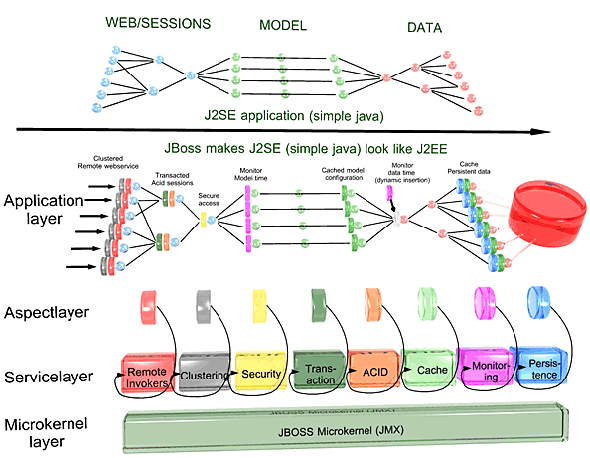
\includegraphics[width=0.8\textwidth]{1.png}

Others are more formal such as these UML (Unified Modeling Language)
diagrams:

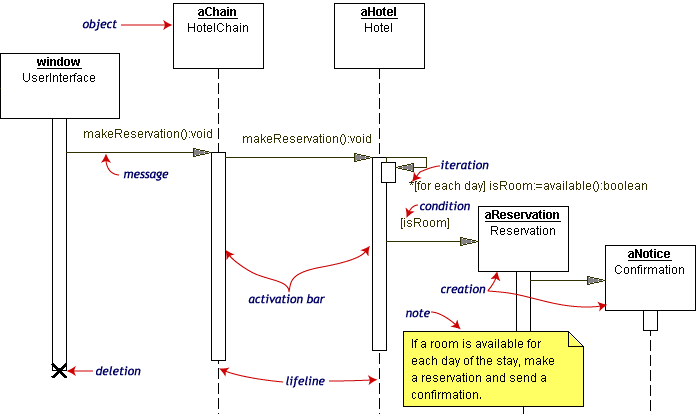
\includegraphics[width=0.8\textwidth]{2.png}

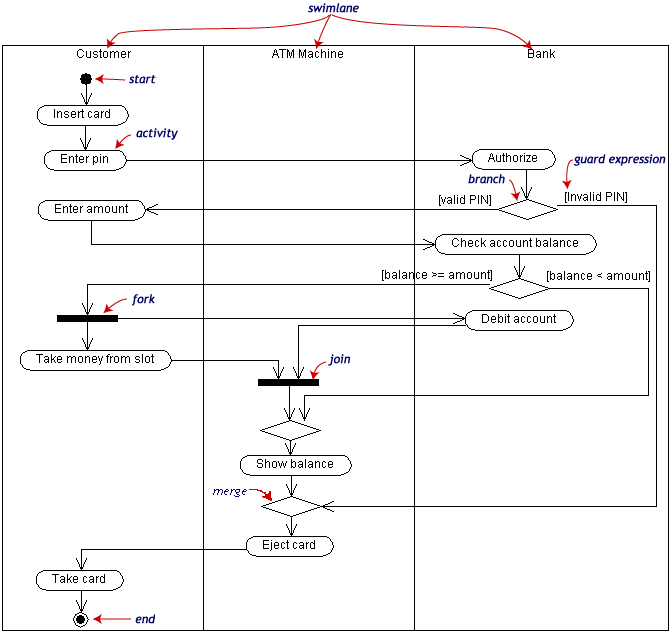
\includegraphics[width=0.8\textwidth]{3.png}

UML is used for an area of study called object-oriented analysis and
design (OOAD) which is an extremely important area of study in software
systems engineering. OOAD is currently the most effective (and most
common) way to analyze and develop software system. Take CISS438
to find out more.
The point is that documentation through the use of high-level diagrams
gives you a different view of the system – usually a higher level overview.
% chapter ends here

\printindex
\end{document}
